\section{Application Scenarios}
\label{sec:caseStudy}
% \shusen{A full case study that driven by the visualization task and the question associated with them}
%In this section, we discuss application scenarios, in which the domain experts utilize the
To illustrate how the proposed perturbation-driven exploration tool helps researchers interpret the neural network model,
we present five interconnected application scenarios domain experts may employ in their analysis workflow.
Users can start the exploration by examining the stability of prediction (Scenario 1), from which they may identify the individual instances worth further investigation (Scenario 2, 3, 4). Alternatively, users can begin with handcrafted common/extreme cases (Scenario 5) and continue from there.
%we present five application scenarios
%(first three roughly correspond to \textbf{T1-3}) gathered by the domain experts who integrated the proposed tool into their analysis workflow.

\begin{figure}[htbp]
\centering
\vspace{-2mm}
 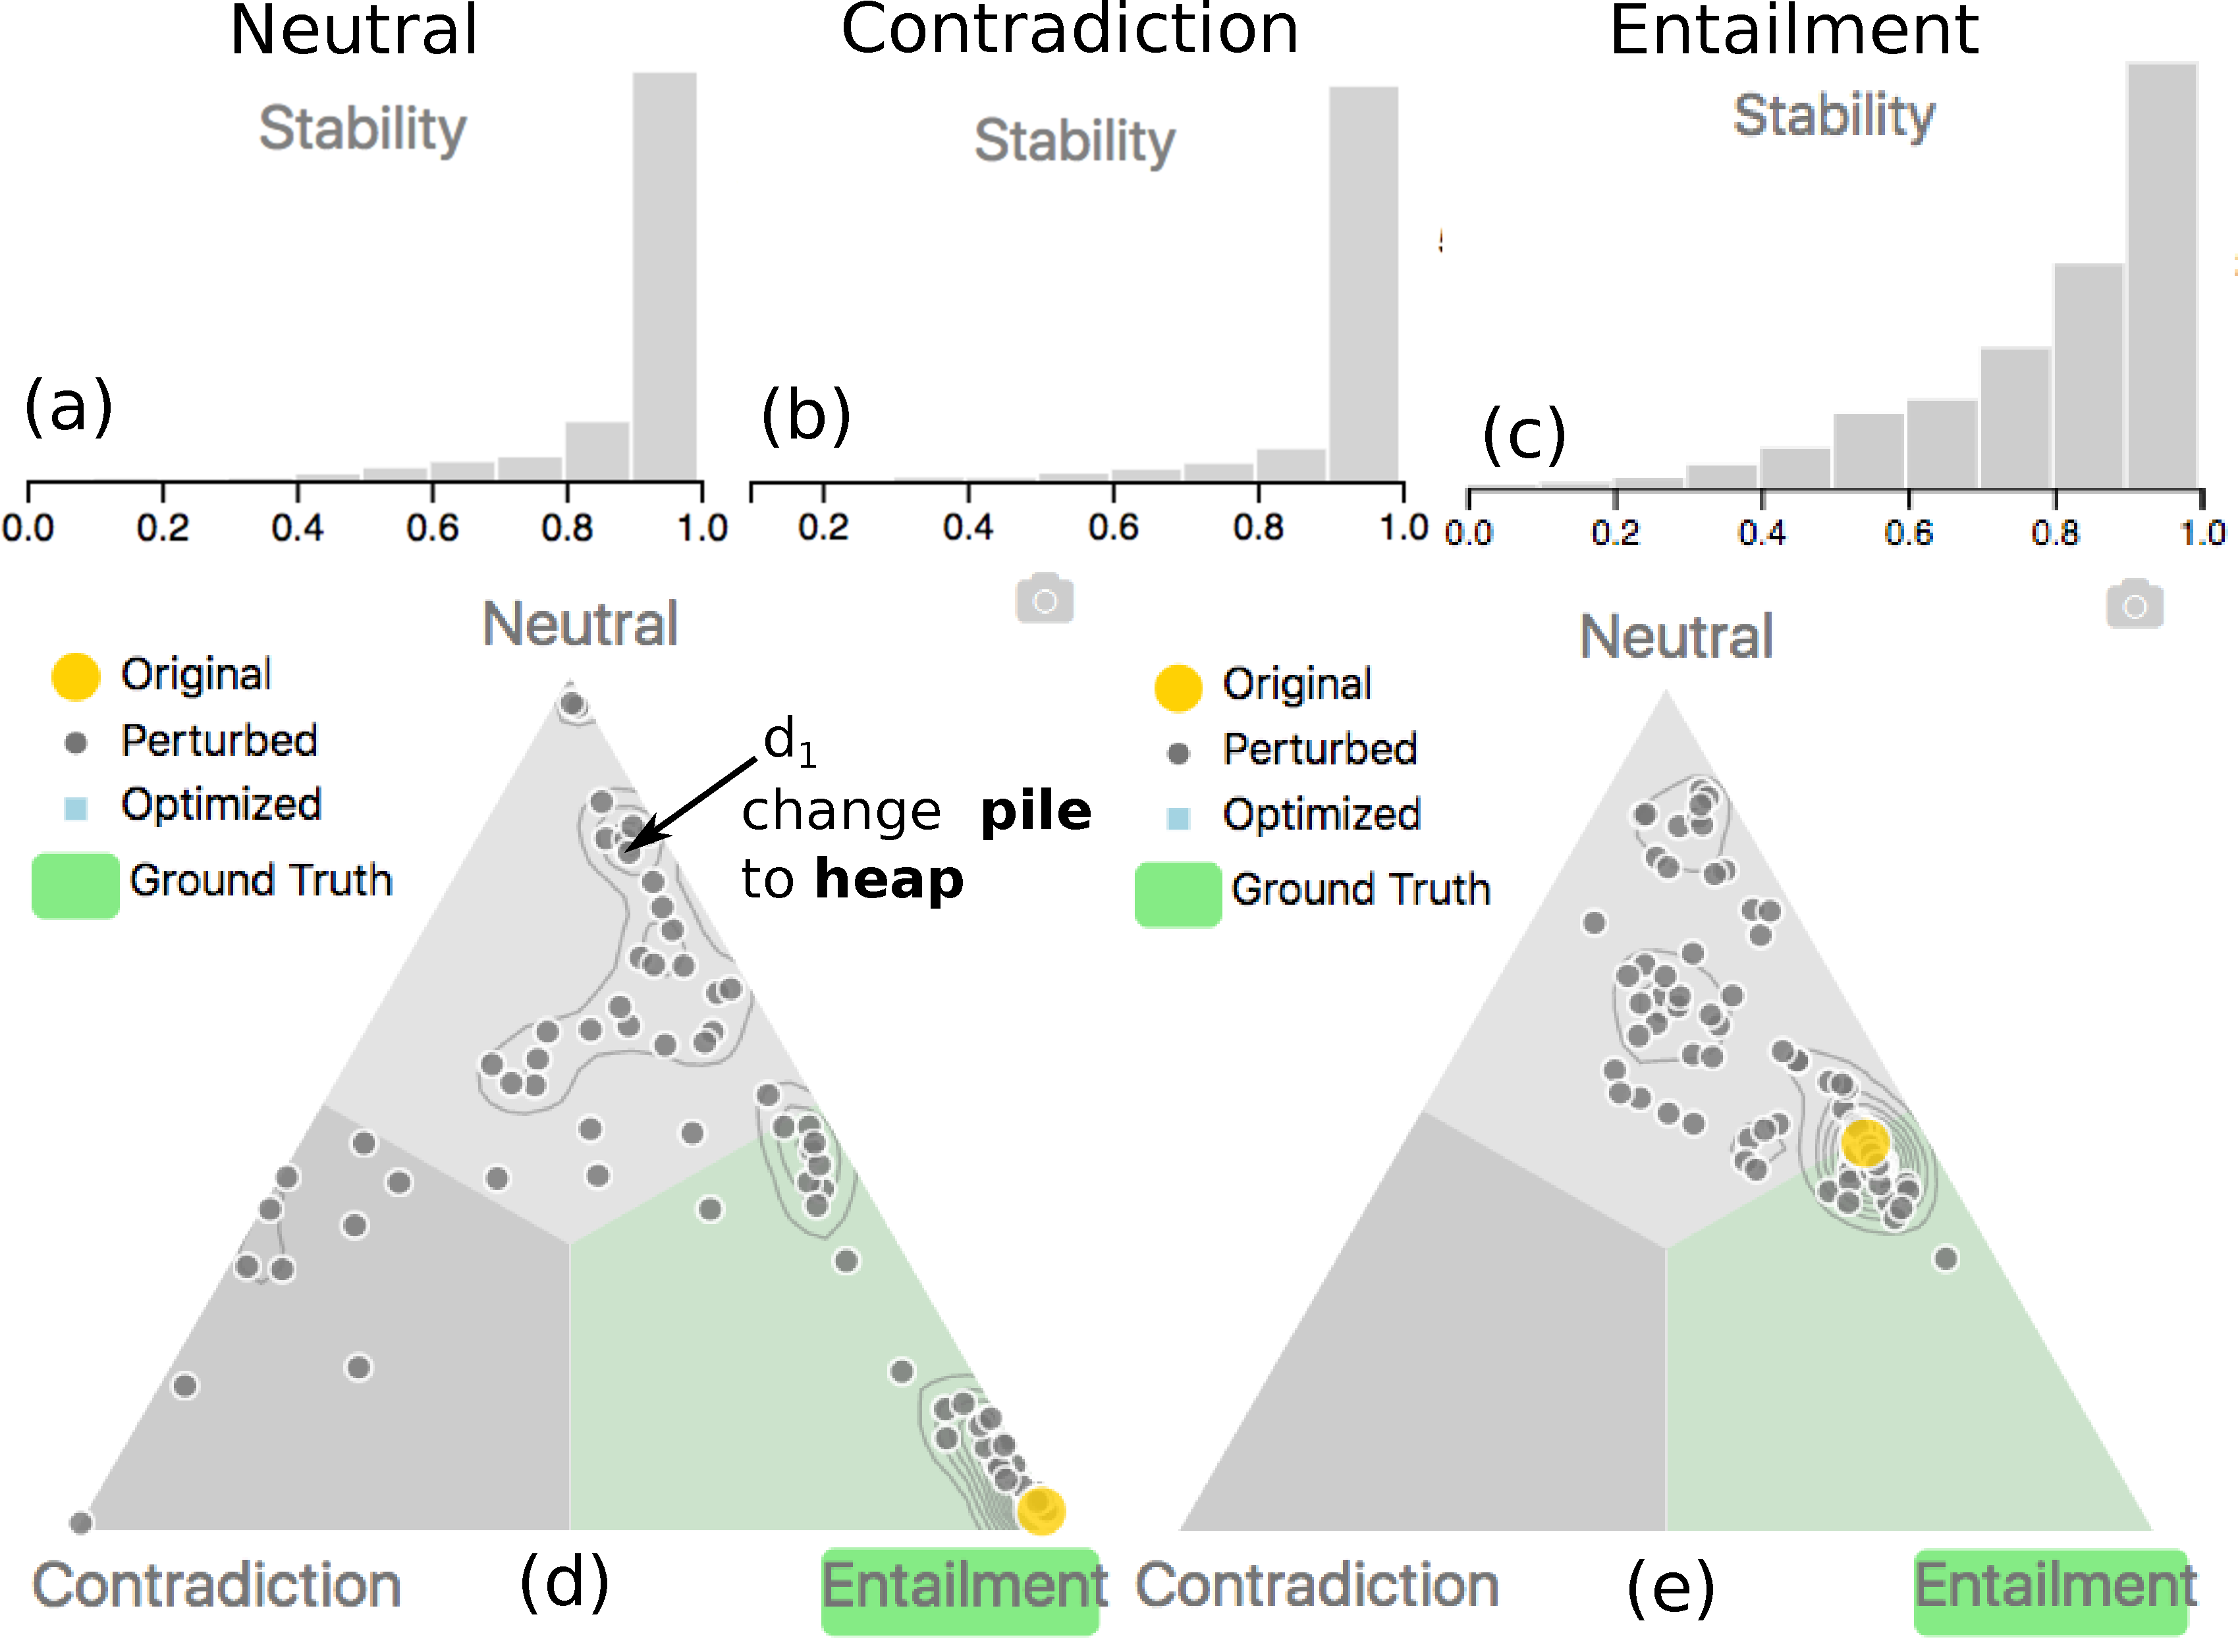
\includegraphics[width=1.0\linewidth]{predictStability}
 \vspace{-6mm}
 \caption{
Prediction stability assessment. In (a)(b)(c), we estimate the overall prediction stability (regarding synonymous perturbation) for each type of prediction over the entire development set (10k examples). The user can drill down to individual examples by using the interface described in Fig.~\ref{fig:summaryView}. In (d), we illustrate a highly unstable prediction, where the original pair's prediction is near a decision boundary (i.e., the yellow circle is between \emph{entailment} and \emph{neutral}). In (e), we show another example of unstable predictions, in which the prediction changes drastically with a minor perturbation (see ($\mathbf{e_1}$)). }
\label{fig:predictStability}
\vspace{-3mm}
\end{figure}

\subsection{Scenario 1: Assess the Model Prediction Stability}
The robustness of the prediction is often hard to evaluate. However, the prediction stability provides valuable information for researchers to better understand the model.
%
In the proposed work, we approach the prediction robustness from a sensitivity analysis point of view. The stability of the prediction is measured by how often the predicted labels are altered after small perturbations are applied to the input.
%
Compared to other types of input (e.g., image), the perturbation of the natural language can be particularly tricky, as small alterations of words can drastically change the meaning of the sentence. As discussed in Section~\ref{sec:sentence}, we try to maintain the sentence semantic by replacing only words with their synonyms and only one word for each pair.
As illustrated in Fig.~\ref{fig:predictStability}, by utilizing the proposed tool, the domain expert can not only examine a visual summary of the stability but also quickly dive into individual examples for a case-by-case analysis.

In Fig.~\ref{fig:predictStability}(a)(b)(c), we compare the overall prediction stability (regarding synonymous perturbation) for all correct predictions in the development set (10k examples in total).
%
We observe a drastic difference for the stability for \emph{entailment} predictions compared to the \emph{contradiction} and \emph{neutral} ones.
%
Such a distinction can be partially explained by how the \emph{entailment} relationship is defined. The relationship is valid only if the concept in the premise is more specific than the concept in the hypothesis. Therefore, the synonymous perturbation may change the \emph{entailment} relationship, as the replaced \emph{noun} or \emph{verb} can be more or less restrictive compared to the original.
This inherent disparity of sensitivity may warrant extra consideration when designing future NLI models.

Besides presenting the summary view, the tool also allows the user to quickly narrow down the selection to a single example by filtering via the histogram and scatterplot (see details in Fig.~\ref{fig:summaryView}).
%
Through the exploration of many samples with low stabilities, domain experts notice that many highly unstable outliers are from sentence pairs where the predictions are near the decision boundary (see Fig.~\ref{fig:predictStability}(d): the yellow circle corresponds to a \emph{entailment} prediction that is very close to \emph{neutral}).
%
However, we can also find sentence pairs, such as the one illustrated in Fig.~\ref{fig:predictStability}(e), in which the prediction is altered drastically with minor perturbations (e.g., replace the word \textbf{pile} with \textbf{heap} in ``pile of snow''). In the following section, we examine what happened inside the model and hypothesize the cause of the failure (see Fig.~\ref{fig:att2pred}).

%%%%%%%%%%%%%%%%%%%%%%%%%%%%%%%%%%%%%%%%%%%%%%%
\begin{figure}[htbp]
\centering
\vspace{-2mm}
 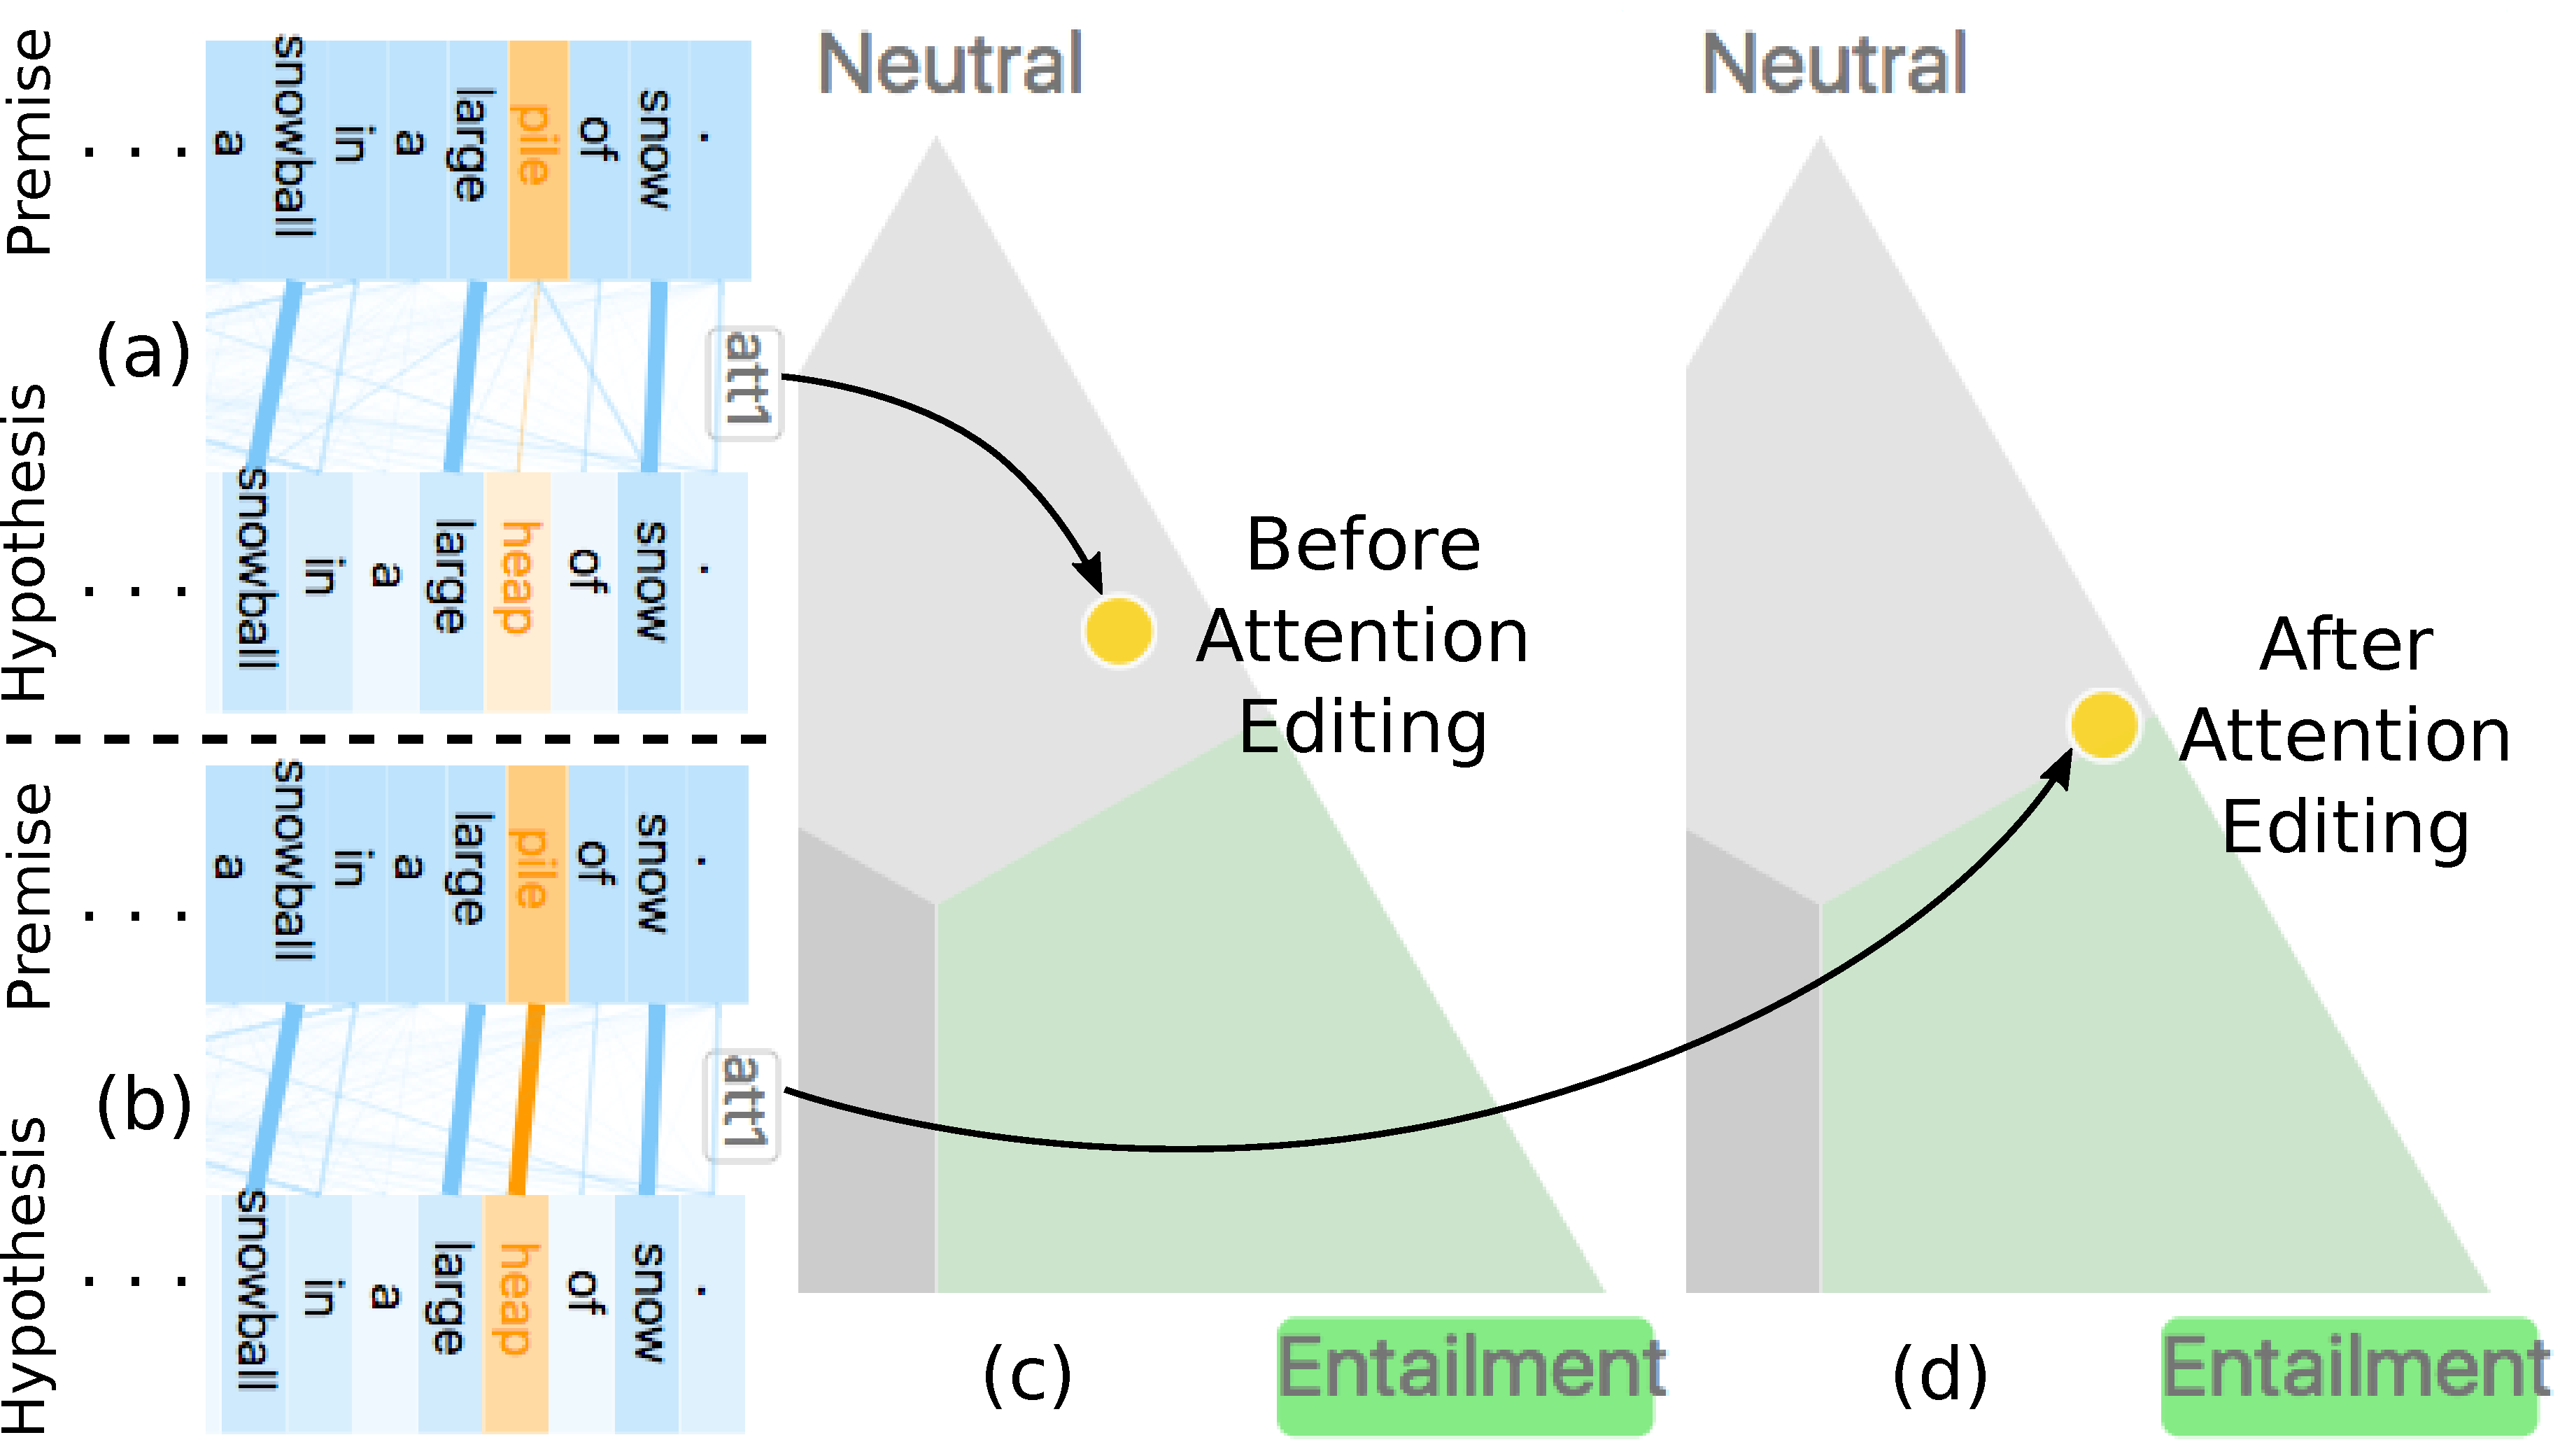
\includegraphics[width=0.9\linewidth]{att2pred}
 \vspace{-4mm}
 \caption{
Editing the original attention (a) to correctly align the word "heap" with "pile" as shown in (b) (these two words are highlighted in orange).
The change of attention leads to the change of prediction from neutral to the class boundary between \emph{neutral} and \emph{entitlement}.
%
}
\label{fig:att2pred}
\vspace{-3mm}
\end{figure}

% perturb input, attention
\begin{figure*}[t]
\centering
\vspace{-3mm}
 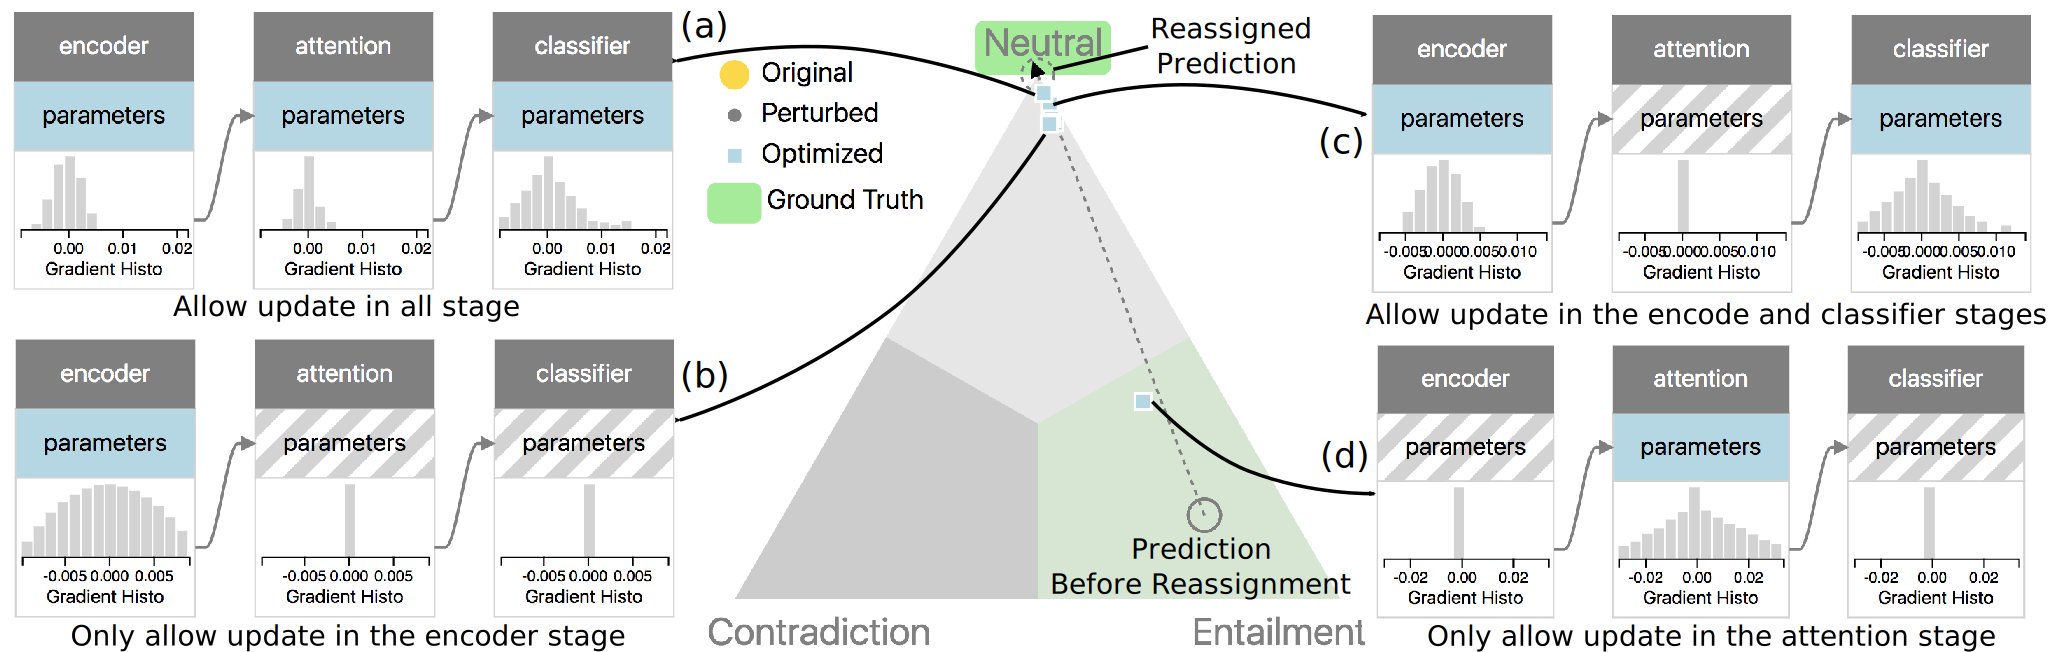
\includegraphics[width=0.95\linewidth]{pipelineUpdate}
  \vspace{-2mm}
 \caption{
Experiment with all configurations for the label reassignment optimization. As shown in (d), the update to the attention stage seems to have significantly less impact on the prediction result compared to the classifier or encoder stage of the model.
 }
  \vspace{-4mm}
\label{fig:pipelineUpdate}
\end{figure*}

\subsection{Scenario 2: Examine the Decision-Making Process}
The predicted label alone provides limited information. Often, domain experts want to know how the model arrives at a conclusion, and if the prediction is incorrect, where in the model the error occurs.
Examining the decision-making process is not only instrumental in evaluating the model performance but also essential for hypothesizing improvement strategies for future models.
%
In the NLI model, the three stages (encoder, attention, classifier) work in synergy to produce the prediction.
Therefore, making sense of the prediction involves understanding how different parts of the model affect the final prediction.

In the previous section, we have noticed that a minor perturbation of the sentence may result a change in the final prediction (Fig.~\ref{fig:predictStability}(e)). Here, we want to make sense of what leads to the failed prediction. In this example, the premise \textbf{P} is ``A very young child in a red plaid coat and pink winter hat makes a snowball in a large \textbf{pile} of snow'', and the original hypothesis \textbf{H1} is ``A child in a red plaid coat and pink winter hat makes a snowball in a large \textbf{pile} of snow''. The perturbed hypothesis \textbf{H2} replaces the word \textbf{pile} with \textbf{heap} in \textbf{H1}. This example should be rather straightforward for the model since there are only minor differences between \textbf{P} and \textbf{H1}/\textbf{H2}.

As illustrated in Fig.~\ref{fig:att2pred}(a), based on the graph attention visualization, we can see in the attention for (\textbf{P}, \textbf{H2}) pair that the words \textbf{pile} and \textbf{heap} are not well aligned.
%
To test whether the alignment is what contributes to the misclassification, the domain expert utilizes the attention editing functionality in the matrix attention view (Fig.~\ref{fig:attentionVis}(c)) to make the word \textbf{pile} align with \textbf{heap} (shown in Fig.~\ref{fig:att2pred}(b)).
%
After the edit, the original prediction (Fig.~\ref{fig:att2pred}(c)) has been moved from neutral to the classification boundary (Fig.~\ref{fig:att2pred}(d)), but the corrected attention fails to produce a conclusive \emph{entailment} prediction (another example, in which the attention edit corrects the final prediction, is shown in Fig.~\ref{fig:depTreeExample}).
%
%Interestingly, the original pair's attention is almost identical to the edited attention (the comparison is not shown in the figure).
Such an observation implies that the model does not firmly believe ``\textbf{heap} of snow'' and ``\textbf{pile} of snow'' have the same meaning, which may indicate a potential issue with the encoder or word embedding.


%\begin{figure}[htbp]
%\centering
%\vspace{-2mm}
% 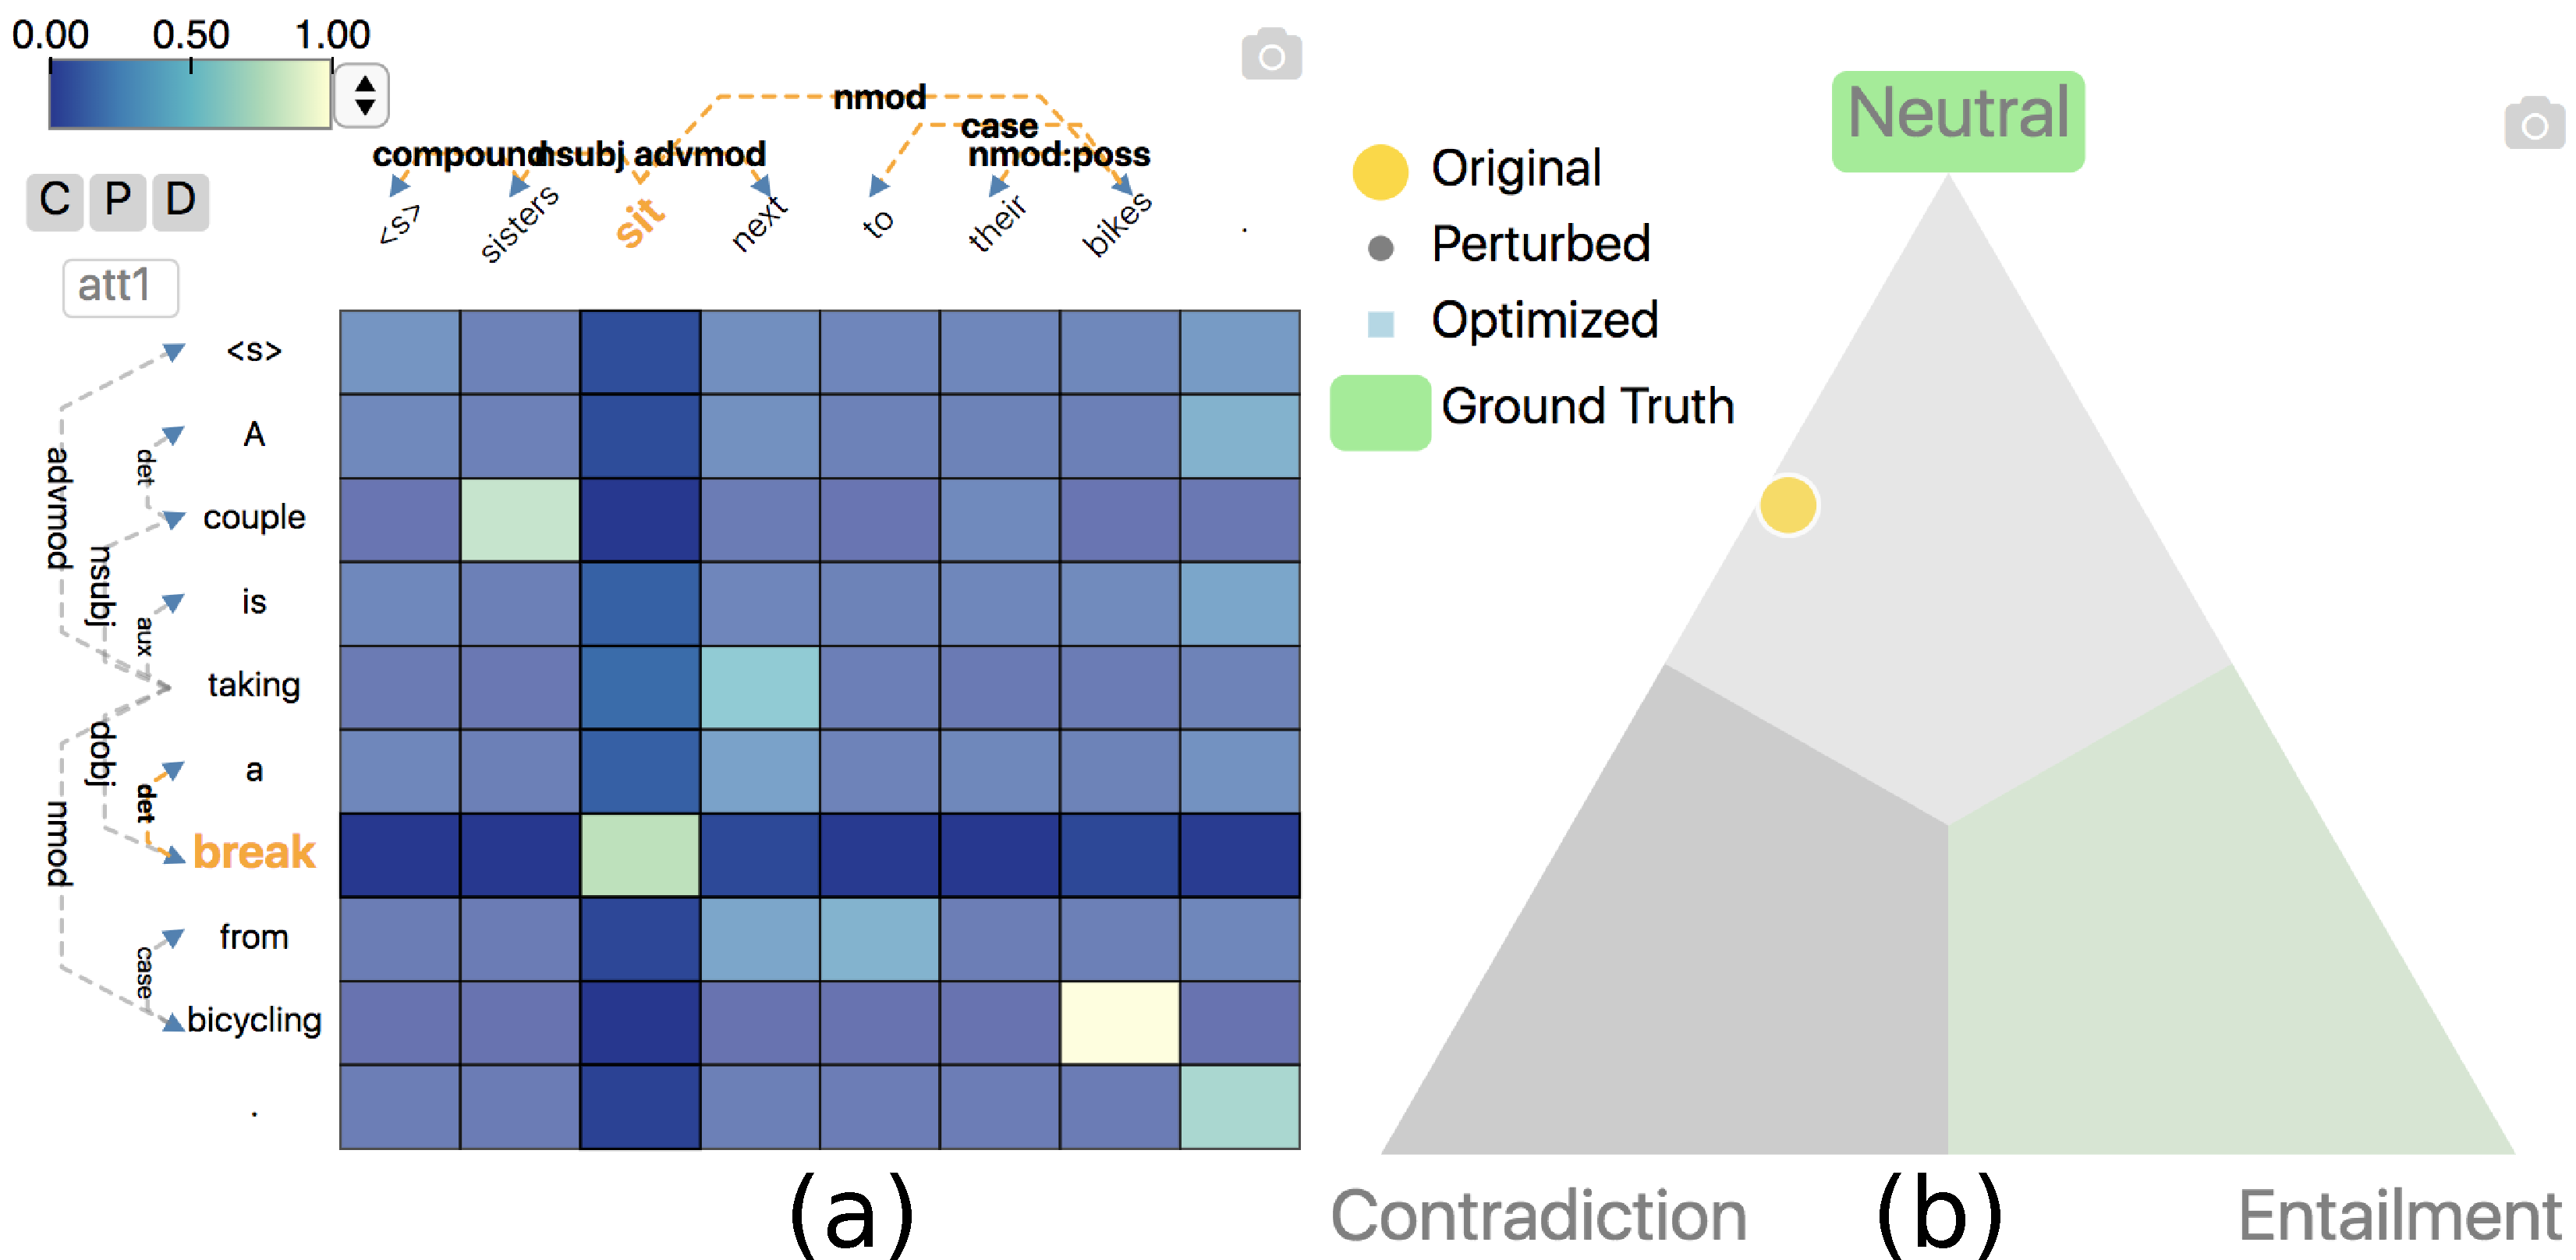
\includegraphics[width=1.0\linewidth]{wrongAlignRightPred}
% \caption{
%The model may produces the right prediction for the ``wrong'' reason, i.e., attention.
%The word \textbf{break} and \textbf{sit} should not align with each other (a). Yet, based on the attention, model still produces the correct prediction (b).
%}
%\label{fig:wrongAlignRightPred}
%\end{figure}


%\shusen{Example where the prediction is correct but the alignment is wrong}
%%%% are we obtain correct prediction from wrong alignment %%%%%
%By looking into the model decision making process, we can assess whether the model is behaving as intended. For the attention based NLI model, one underlying assumption is that the attention should capture the correct alignment between words in the premise and hypothesis sentence for the classifier to make an informed/correct decision.
We have shown that the perfect alignment does not necessarily guarantee a correct prediction.
%
On the flip side, we may produce the right predictions for the ``wrong'' reason (i.e., incorrect attention).
%As illustrated in Fig.~\ref{fig:wrongAlignRightPred},
For example, in the sentence pair (\textbf{P}: ``A couple is taking a break from bicycling'', \textbf{H}: ``sisters sit next to their bikes''), the words \textbf{take} and \textbf{next} should not align with each other,
yet the model still predict the correct label (\emph{neutral}).% (Fig.~\ref{fig:wrongAlignRightPred}(b)).

%By looking into the model decision making process, we can assess whether the model is behaving as intended.
%These situations demonstrate the important of understanding the model decision making process, we can assess whether the model is behaving as intended.


%%%% hypothesis on which part of model is wrong? %%%%%


%One of the essential task for can be made in either of these stages.
% \shusen{difference in sensitivity among entail natural and contradict relationships}
% the generate the correct prediction for the wrong reason


%%%%%%%%%%%%%%%%%%%%%%%%%%%%%%%%%%%%%%%%%%%%%%%
\subsection{Scenario 3: Update the Model to Correct a Prediction}
%\subsection{Scenario 3: What Does It Take to Correct a Failed Prediction?}
Up to here, we have employed perturbation for input to understand prediction robustness and utilized the perturbation of attention (and input) to infer the model decision-making process. Both these perturbation operations rely on forward propagation in the pipeline and assume the model parameter remains unchanged.
%
However, once we get a sense of how predictions are made and hypothesize about the cause of the failure in the case of a prediction error, it is natural to ask follow-up questions: What does it take to fix an incorrect prediction? And more importantly, what role does each of the three stages play in such a process? And, are they affecting the prediction differently?

Domain experts can obtain answers to these questions by utilizing the prediction and pipeline view in the proposed tool. As discussed in detail in Section~\ref{sec:pipeline}, we employed a margin-infused relaxed algorithm (MIRA) based optimization with two objectives (apply the least amount of change to the parameter, and make the new prediction as close to the reassigned prediction as possible) to update the network parameters.
%
We then visualize how much each stage of the model is changed through the distribution of differences between the two sets of parameters (see Fig.~\ref{fig:pipelineView}).

To infer the role each stage of the pipeline plays, the proposed tool allows the parameter update to be enabled or disabled for each pipeline stage.
The system also includes an automatic option to test all the possible configuration combinations. As illustrated in Fig.~\ref{fig:pipelineUpdate}, the ground truth for this sentence pair is \emph{neutral}. However, the model produces an incorrect label \emph{entailment}. The domain expert reassigns the prediction to \emph{neutral}, which triggers the prediction update optimization for seven different pipeline configurations. Four configurations are shown in Fig.~\ref{fig:pipelineUpdate}(a)(b)(c)(d). The updated predictions are illustrated as blue squares, and the arrowed lines highlight the corresponding pipeline configurations.

Interestingly, all configurations except one are concentrated around the full \emph{neutral} prediction. Referring back to the pipeline visualization, we observe that the only configuration that failed to produce the correct label is the one for which we allow only updating of the attention stage of the model.
%
%In other words, the updating of the attention stage seems to have significantly less impact on the prediction result compared to the classifier or encoder stage of the model.
%Similar observations can be obtained for most examples we have experimented with.
%\shusen{
%The domain experts comment that this observation is interesting and worth further investigation from the perspective of NLP research.
%The domain experts find this observation very interesting and suggest a preliminary interpretation. They believe the attention provides a way to compose word semantics. Individual word semantics are yielded from the encoder and input embedding, while the composed semantics participate in classification layer. From this analysis, we can extrapolate that adjusting the word alignment affects only the composed semantics but has no effect on word semantics, which often plays a significant role in a good model (as supported by recent works in word embeddings, e.g., ELMo~\cite{salant2017contextualized}). Without proper semantics (in both encoder and classifier), only adjusting alignment is not sufficient to yield good model. 
%
The domain experts find this observation very interesting and suggest a preliminary interpretation. The reason, as they believe, is that the attention layer functions differently from the encoder and the classifier in terms of word semantics. The attention layer in this model is more specialized in composing word semantics rather than creating new semantics. When it comes to fixing a wrong prediction, attention layer affects the prediction less significantly while the encoder and the classifier can swiftly adapt to the correct label. Thus from this analysis, we can extrapolate that the ultimate prediction relies on the semantics (i.e., encodings and composed encodings in the classifier). Recent word embeddings works (e.g., ELMo~\cite{salant2017contextualized}) also support such an observation that better word embeddings can substantially benefit a model. However, the result by no means implies attention is not useful, because it serves as a way to compose word semantics.
%To interpret the result, we need to carry out a case by case analysis, as the separation of the stages depends on the individual implementation.
%In our case, the result indicates that the tunable parameters of the attention stage (the transformation before the alignment operation, see details in Appendix A) has less impact on the final prediction compared to the other two stages.
%However, this result does not necessarily imply the limitation of attention mechanism as the core alignment computation does not have tunable parameters that can be modified by the proposed optimization.
%}
%The attention layer is less sensitive compared to encoding layer and classification layer.
%When examined other sentences pairs, such an observation remains.
%This gives domain expert some hint about the significance of the role of each pipeline stage play in this model.
% which based on the natural extension of the margin-infused relaxed algorithm (MIRA) to the neural network generalize the concept of maligin combined effort of the  proposed technique

%
%However, to understand how the model should
\begin{figure*}[t]
\centering
\vspace{-2mm}
 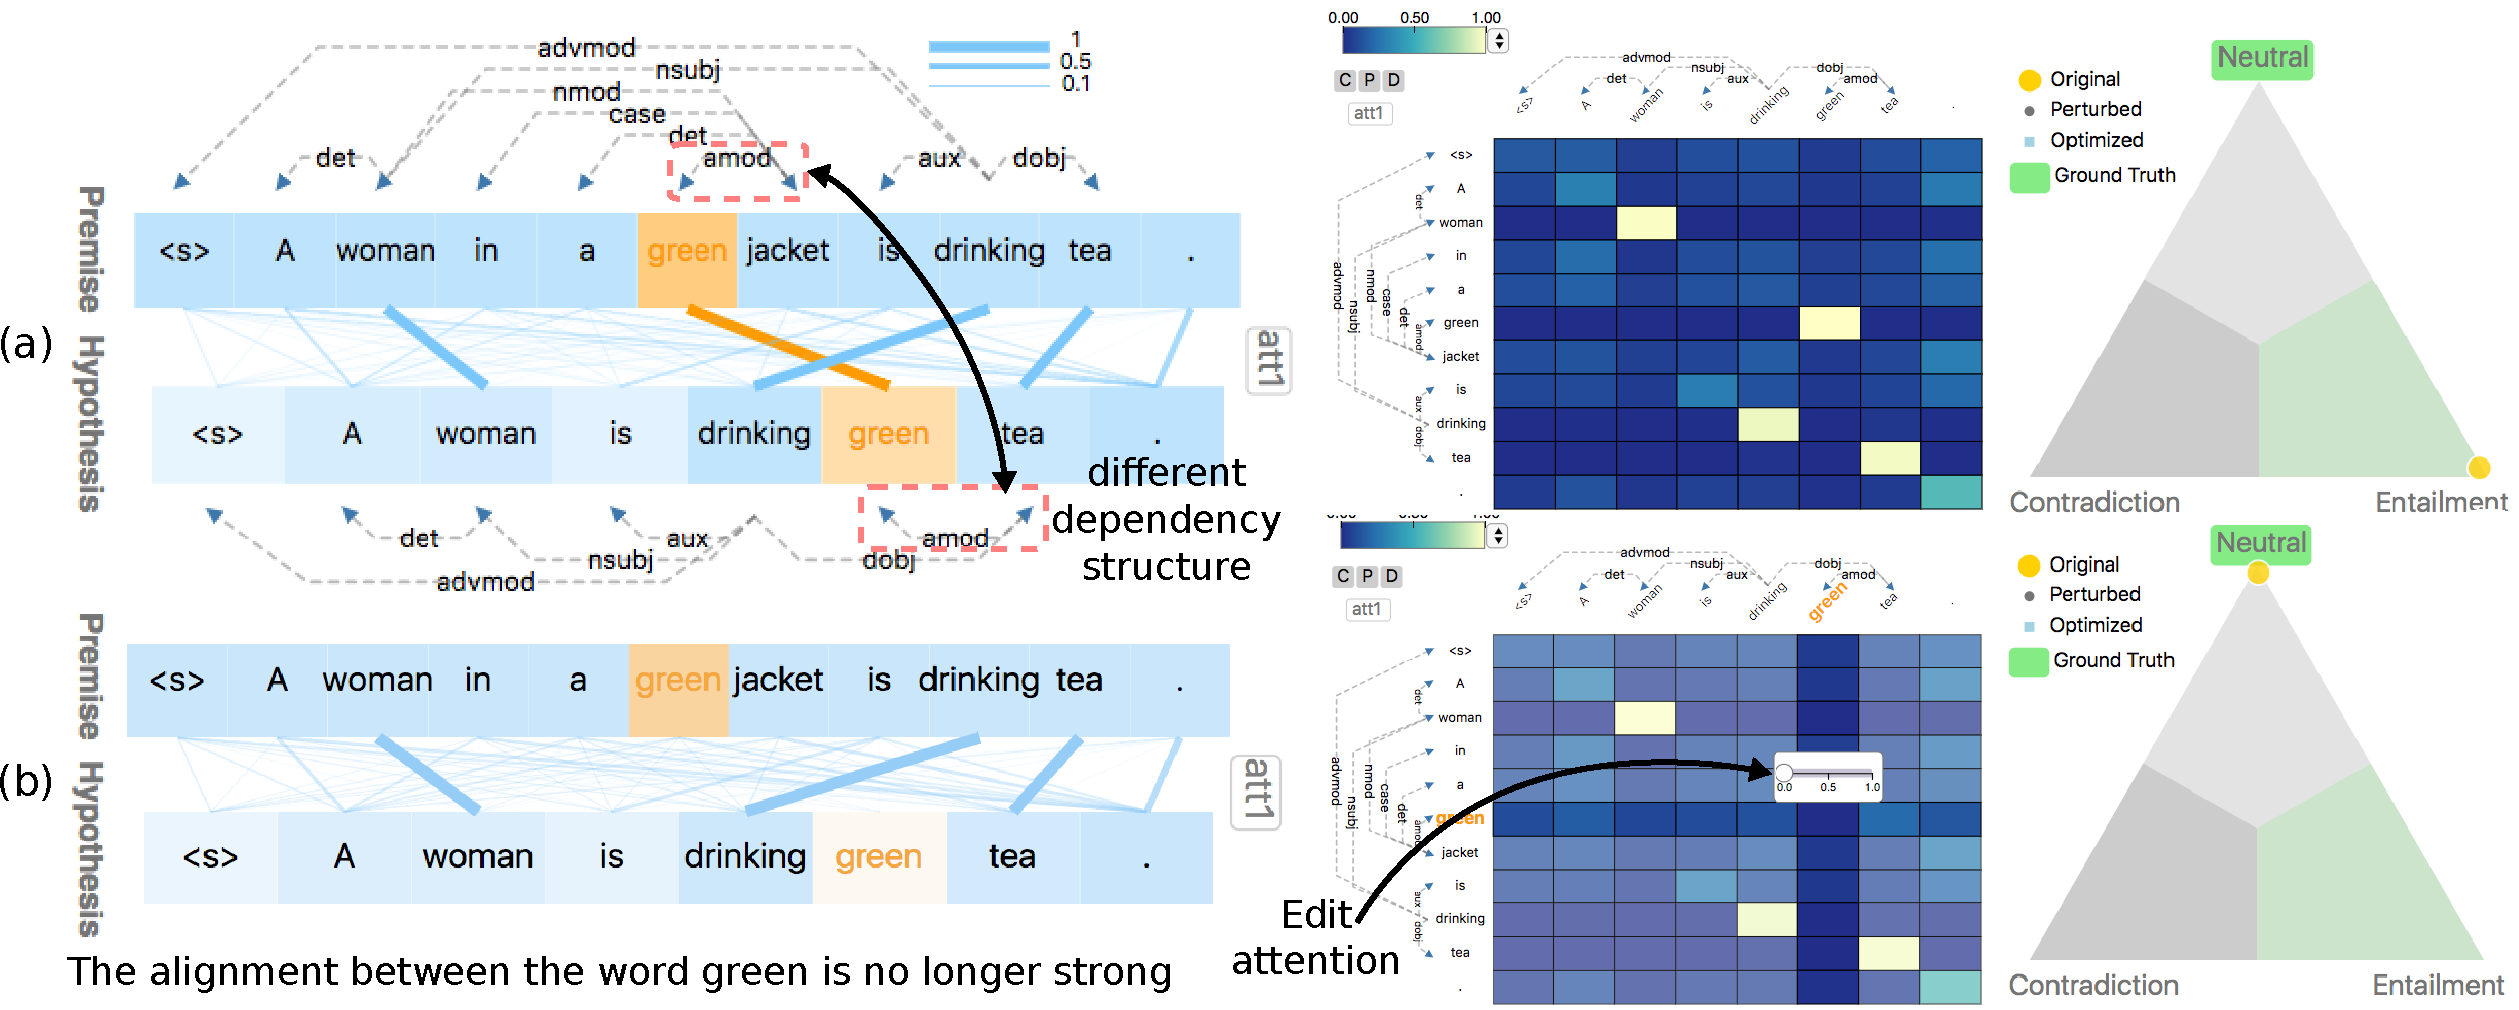
\includegraphics[width=0.98\linewidth]{DepTreeExample}
  \vspace{-3mm}
 \caption{
The dependency tree provides valuable information that can help fix the prediction error.
In (a), the model mistakenly aligns the word green, which leads to an incorrect prediction.
After examining the dependency tree (highlighted by pink squares), we can see the two \textbf{greens} are attached to different words.
In (b), by editing the attention and forcing the alignment of the two \textbf{greens} to be zero, the prediction label is corrected to \emph{neutral}.
 }
\label{fig:depTreeExample}
 \vspace{-4mm}
\end{figure*}

%%%%%%%%%%%%%%%%%%%%%%%%%%%%%%%%%%%%%%%%%%%%%%%
\subsection{Scenario 4: Explore the Relationship Between Grammar and Attention}
\label{sec:grammarAttention}
The attention computation in the NLI model does not take the grammar structure of the sentences into consideration,
yet the attention often highlights key elements of the sentence.
Therefore, domain experts wish to understand whether attention alone is sufficient to capture sentence structure;
and, more importantly, what kind of additional information from grammar parsing can help address the NLI challenge.

In the proposed system, we overlay the sentence dependency tree with the attention, which enables researchers to conduct comparisons between attention and grammar structure.
As illustrated in Fig.~\ref{fig:depTreeExample}(a), the prediction of the sentence pair (\textbf{P}: ``A woman in a green jacket is drinking tea.'' \textbf{H}: ``A woman is drinking green tea.'') is wrong. We can infer the cause by examining the attention, in which the word \textbf{green} in ``\textbf{green} jacket" is aligned to the \textbf{green} in ``\textbf{green} tea". Due to such an alignment, the model mistakenly believes the two \textbf{greens} are used to describe the same thing (therefore, predict \emph{entailment}).  However, as we examine the dependency tree, the two \textbf{greens} are attached to different words, i.e., \textbf{green} in \textbf{P} is attached to ``jacket'', whereas \textbf{green} in \textbf{H} is attached to ``tea''. Therefore, they should not be aligned to allow the classifier to make the right decision.
%
This experiment demonstrates the potential benefit of including grammar structure in the alignment computation. %This stresses the importance of dependency tree in our tool.
%
Interestingly, as illustrated in Fig.~\ref{fig:depTreeExample}(b), by editing the attention and forcing the alignment of the two \textbf{greens} to be zero, the prediction label is corrected (\emph{neutral}).

%%%%%%%%%%%%%%%%%%%%%%%%%%%%%%%%%%%%%%%%%%%%%%%
\subsection{Scenario 5: Handcrafted Example Exploration}
To test the limits of the model, domain experts often handcraft ``extreme'' examples (such as the Facebook IPO example discussed in Section~\ref{sec:languageInference}) for which they know most models will have difficulty making a correct inference.
%
The researchers start with a set of experiments they plan to run, from which they will develop new hypotheses for further analysis.
%
We can think of such a process as a natural blend of all previously discussed scenarios. However, instead of having a specific goal in mind, the domain experts focus on probing around to uncover any interesting or out-of-the-ordinary behaviors in the model.
%


%\subsection{Is the Prediction Stable?}
%\subsection{Where Are the Mistakes?}
%\subsection{How Attention Affect the Prediction?}
%\subsection{What Does It Take to Change the Prediction?}
%\subsection{Is Attention All You Need?}
